\documentclass{article}
\usepackage{fancyhdr}
\usepackage{ctex}
\usepackage{listings}
\usepackage{graphicx}
\usepackage[a4paper, body={18cm,22cm}]{geometry}
\usepackage{amsmath,amssymb,amstext,wasysym,enumerate,graphicx}
\usepackage{float,abstract,booktabs,indentfirst,amsmath}
\usepackage{array}
\usepackage{booktabs}
\usepackage{multirow}
\usepackage{url}
\usepackage{diagbox}
\renewcommand\arraystretch{1.4}
\usepackage{indentfirst}
\setlength{\parindent}{2em}
\usepackage{enumitem}
\setmonofont{Consolas}
\usepackage{listings}
\usepackage{xcolor}
\usepackage{makecell}
\usepackage{tikz}
\usetikzlibrary{positioning, arrows.meta}
\setCJKmonofont{黑体}
\lstset{  
	% 基本设置  
	xleftmargin = 3em, xrightmargin = 3em, aboveskip = 1em,  
	backgroundcolor = \color{white},  
	basicstyle = \small\ttfamily,  
	rulesepcolor = \color{gray},  
	breaklines = true,  
	numbers = left,  
	numberstyle = \small,  
	numbersep = -14pt,  
	frame = shadowbox,  
	showspaces = false,  
	columns = fixed,  
	sensitive = true,  
	% VSCode 风格配色  
	keywordstyle = \color{blue!70!black}\bfseries,  
	emphstyle = \color{red!70!black}\bfseries, % 对于强调的词  
	emphstyle=[2]\color{purple!70!black}\bfseries, % 对于第二组强调的词  
	commentstyle = \color{green!60!black}, % 注释颜色  
	stringstyle = \color{orange!90!black}, % 字符串颜色更亮一些  
	morekeywords={ASSERT, int64\_t, uint32\_t},  
	moreemph={ASSERT, NULL},  
	moreemph=[2]{int64\_t, uint32\_t, tid\_t, uint8\_t, int16\_t, uint16\_t, int32\_t, size\_t, bool},  
	morecomment=[l][\color{green!60!black}]{+}, % 以+开头的注释  
}

%--------------------页眉--------------------%
\pagestyle{fancy}
\fancyhead[L]{}
\fancyhead[R]{}
\fancyhead[C]{华东师范大学软件工程学院实验报告}
\fancyfoot[C]{-\thepage-}
\renewcommand{\headrulewidth}{1.5pt}
%--------------------标题--------------------%
\begin{document}
\begin{center}
	{\Large{\textbf{\heiti 华东师范大学软件工程学院实验报告}}}
	\begin{table}[H]
		\centering
		\begin{tabular}{p{2cm}p{4cm}<{\centering}p{1cm}p{2cm}p{6cm}<{\centering}}
			课程名称:    & 操作系统实践 & \quad & 指导教师:    & 张民
			\\ \cline{2-2} \cline{5-5}
			姓\qquad 名: & 王海生    & \quad & 学\qquad 号: & 10235101559         \\ \cline{2-2} \cline{5-5}
			实验编号:    & 实验四 & \quad & 实验名称:    & 修改忙等
			\\ \cline{2-2} \cline{5-5}
		\end{tabular}
	\end{table}
	
	% 添加新行并居中
	%\vspace{1em} % 可选:添加垂直间距
	\textbf{代码仓库:}\url{https://github.com/Hanson-Wang-chn/ECNU-Operating-System-WHS.git}
\end{center}
\rule{\textwidth}{1pt}
%--------------------正文--------------------%
\section{实验目的}

\begin{enumerate}
	\item 展示忙等:在函数\texttt{thread\_yield()}中添加\texttt{print}语句打印必要信息,运行指令\texttt{pintos -v -- -q run alarm-multiple},查看展示运行结果,并文字说明其是忙等;
	
	\item 实现休眠:实现\texttt{thread}的\texttt{sleep}功能,在wake up时添加\texttt{print}语句打印必要信息,再次运行指令\texttt{pintos -v -- -q run alarm-multiple},查看展示新的运行结果,以及和之前结果的差别,并文字说明其原因;
	
	\item 实现苏醒后抢占:\texttt{sleep}的进程醒来时,如果当前running的进程优先级比它低,醒来的进程抢占执行。可以回忆上一次的实践课内容关于priority的内容。
\end{enumerate}

\normalsize

\section{实验内容与设计思想}

在\texttt{src/threads/}目录下运行\texttt{make check},可以看到有下面几个测试点:

\begin{lstlisting}
	pass tests/threads/alarm-single
	pass tests/threads/helloworld
	pass tests/threads/alarm-multiple
	pass tests/threads/alarm-simultaneous
	FAIL tests/threads/alarm-priority
	pass tests/threads/alarm-zero
	pass tests/threads/alarm-negative
\end{lstlisting}

\begin{enumerate}
	\item 展示忙等:在函数\texttt{thread\_yield()}中添加打印语句,用于输出当前线程名称及其被调度时的系统tick数。通过执行\texttt{pintos -v -- -q run alarm-multiple}命令,并观察输出结果,可以发现系统频繁地进行上下文切换,即使某些线程没有实际工作需要处理。这表明原始实现采用了效率较低的忙等待机制来处理休眠请求。
	
	\item 实现休眠:为了优化休眠机制,我们需要重新实现\texttt{timer\_sleep()}函数。新的实现方式是将请求休眠的线程放入一个专门的等待队列\texttt{wait\_list}中,并为每个线程设置了一个预计唤醒时间点\texttt{wake\_tick}。每当系统经过一个tick时,仅需检查\texttt{wait\_list}中的第一个元素是否达到了预定的唤醒时刻。如果条件满足,则将该线程从\texttt{wait\_list}移除并加入到就绪队列\texttt{ready\_list}中准备执行。此外,在每次线程被唤醒时也加入了相应的打印信息,以便于后续分析线程的实际行为模式变化。通过再次运行\texttt{pintos -v -- -q run alarm-multiple}命令,可以看到新机制下的输出结果更加有序,减少了不必要的CPU资源消耗。
	
	\item 实现苏醒后抢占:为了让系统能够根据优先级进行更灵活的调度,我们需要对\texttt{thread\_unwait()}函数进行调整。当高优先级的线程从休眠状态恢复且发现当前正在执行的线程具有较低优先级时,新唤醒的线程会立即获得处理器控制权。为此,我们在检测到有线程被唤醒后设置了标志变量\texttt{yield\_flag},并通过\texttt{intr\_yield\_on\_return()}确保在中断返回时触发一次强制性的上下文切换尝试。这样,不仅增强了Pintos操作系统对于睡眠/唤醒操作的支持,同时也强化了其按照优先级进行调度的能力,使得整个系统更加高效和响应迅速。
\end{enumerate}

\normalsize

\section{使用环境}

\subsection{主机系统配置}

本次实验的主机系统环境如下表所示:

\begin{center}
	\begin{tabular}{| >{\centering\arraybackslash}m{3cm} | >{\centering\arraybackslash}m{7cm} |}    
		\hline  
		\textbf{项目名称} & \textbf{详细信息} \\
		\hline  
		操作系统 & macOS Sequoia 15.0 \\  
		\hline  
		系统类型 & 64位操作系统,基于ARM的处理器 \\  
		\hline
		CPU & Apple M1 Pro \\  
		\hline 
		GPU & Apple M1 Pro\\  
		\hline 
		内存 & 16GB 统一内存 \\  
		\hline 
		磁盘 & 512GB SSD \\  
		\hline 		
	\end{tabular}
\end{center}

\subsection{Docker配置}

在官网下载并安装后,Docker容器正常运行,如下图所示:

\begin{figure}[H]
	\centering
	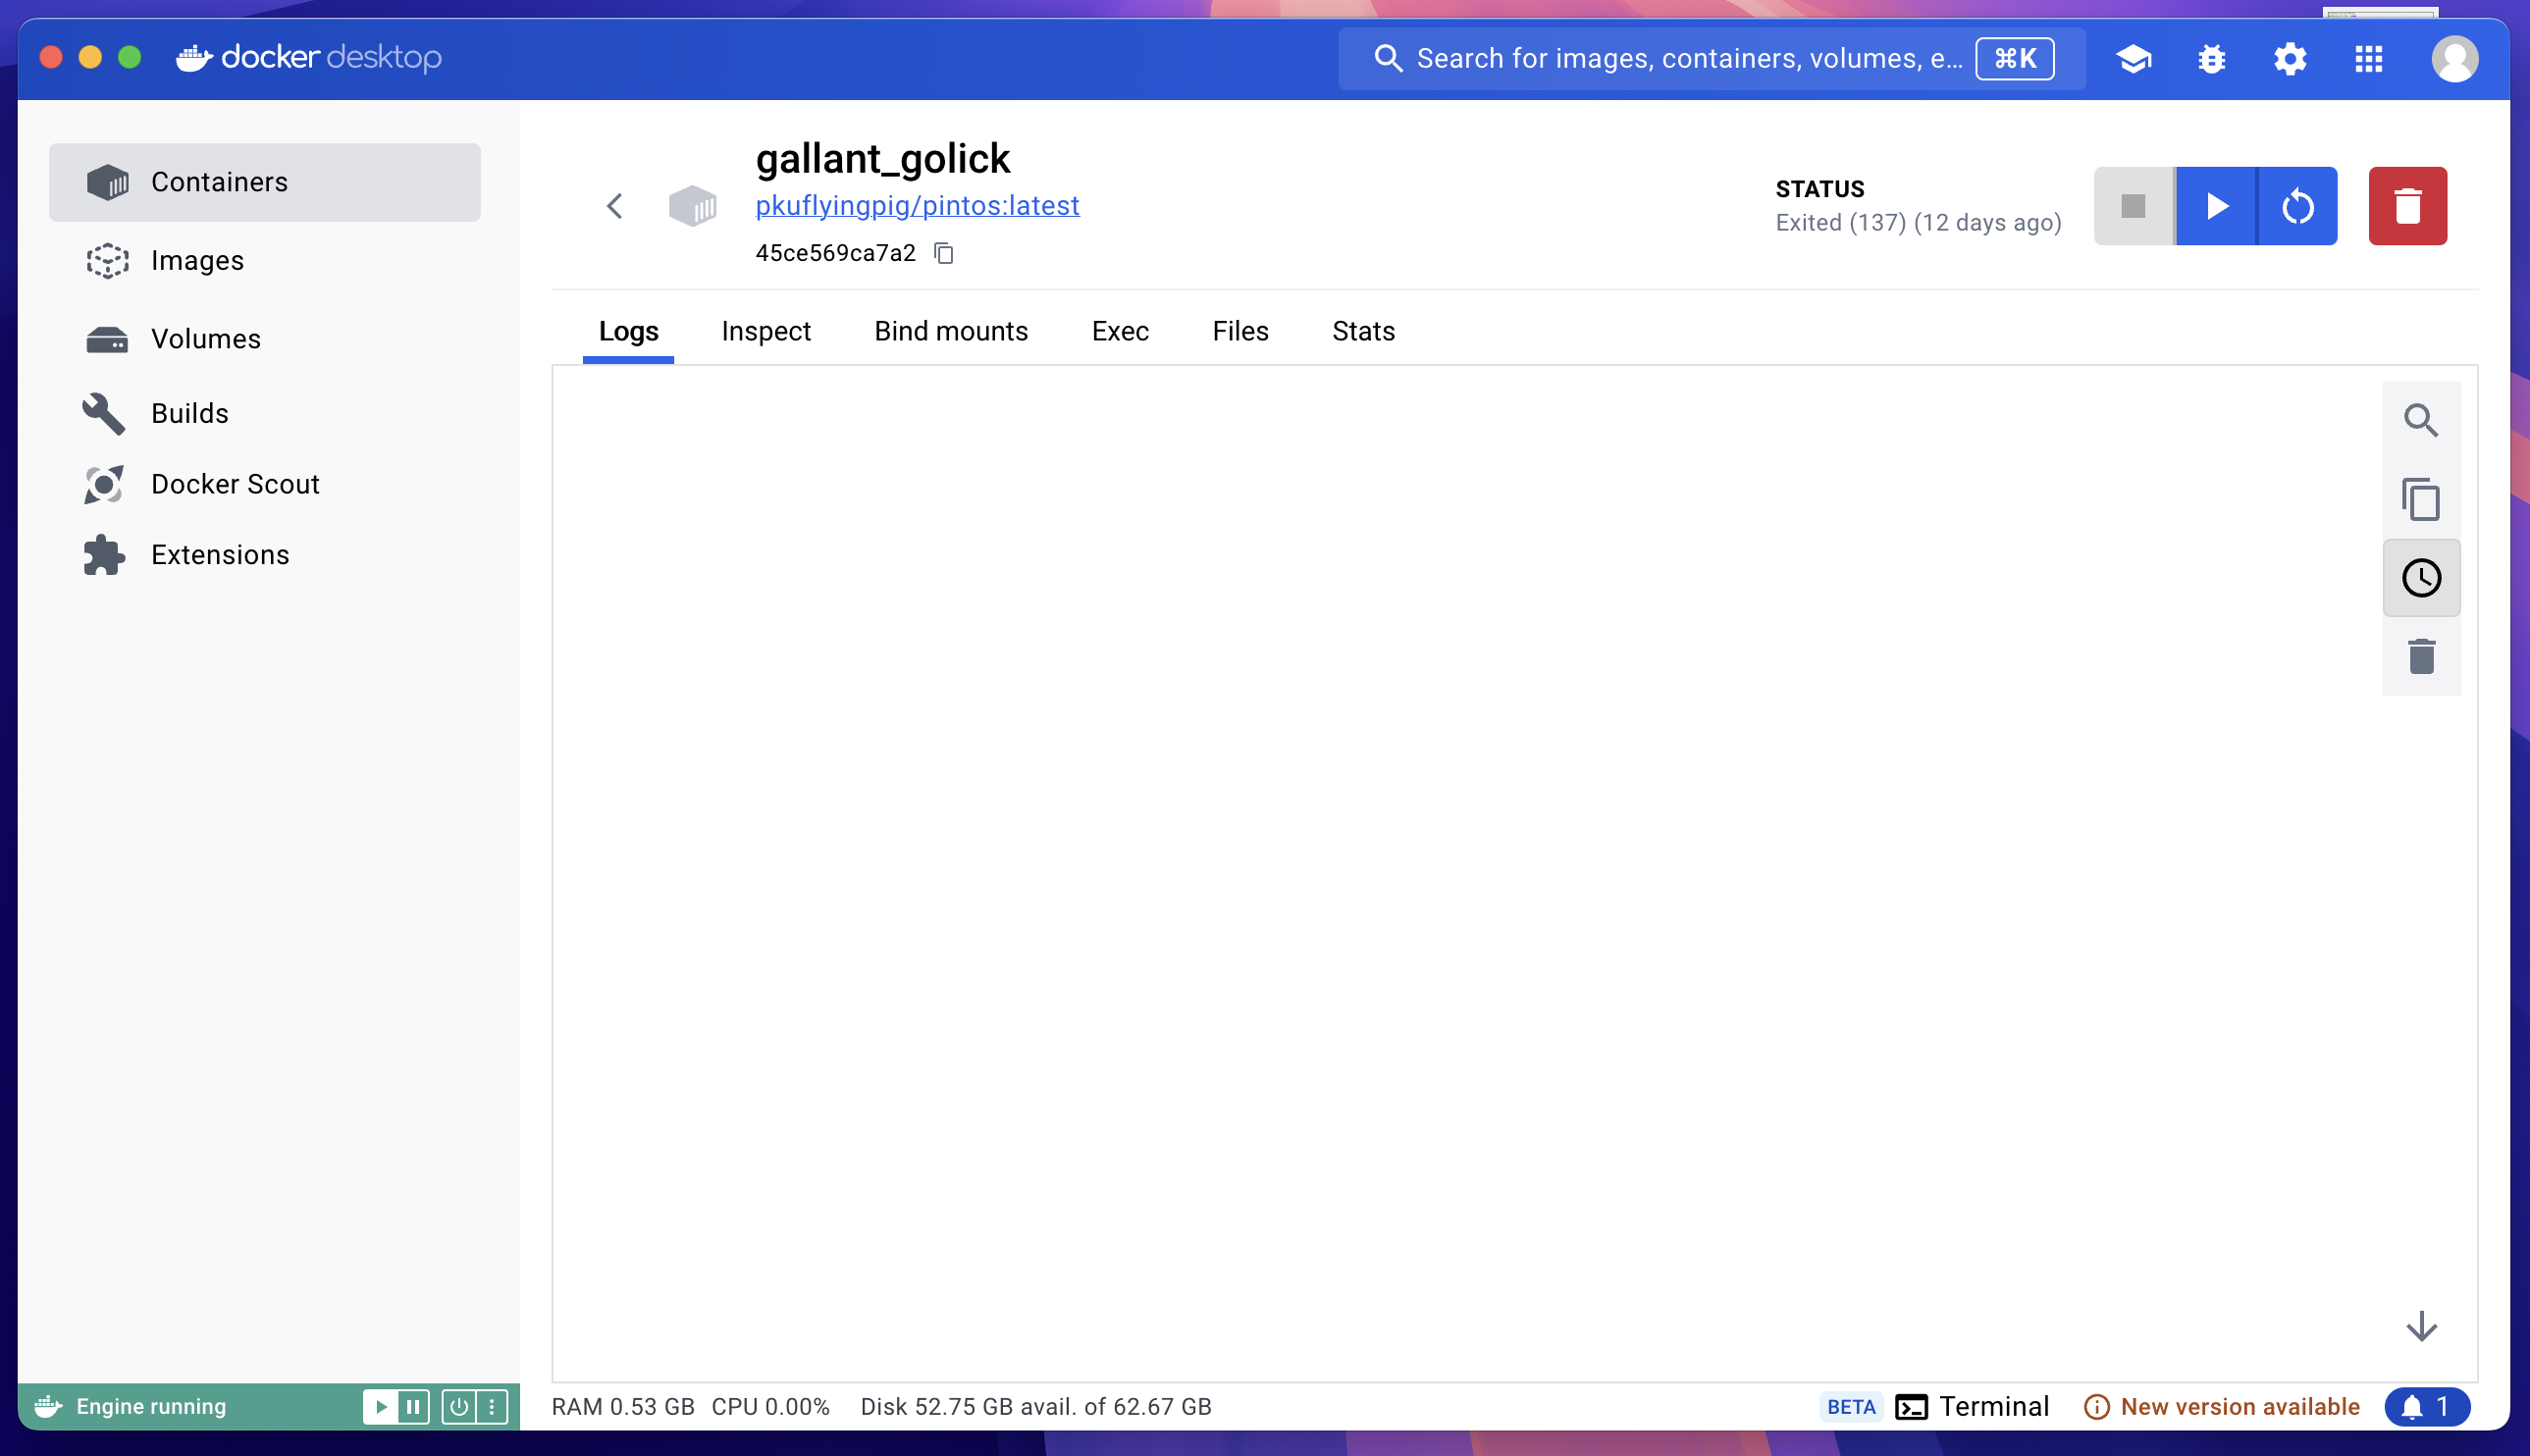
\includegraphics[width=0.9\textwidth]{img/docker_install.png}
	\caption{Docker容器}
\end{figure}

接着使用下面的命令实现磁盘挂载,方便文件管理:

\begin{lstlisting}[language=Bash, title=启动Docker容器并挂载文件]
	docker run -it --rm --name pintos --mount type=bind,\
	source=/Users/wanghaisheng/Desktop/Coding/ECNU-Operating-System-WHS/pintos,\
	target=/home/PKUOS/pintos pkuflyingpig/pintos bash
\end{lstlisting}

完成后如下图所示:

\begin{figure}[H]
	\centering
	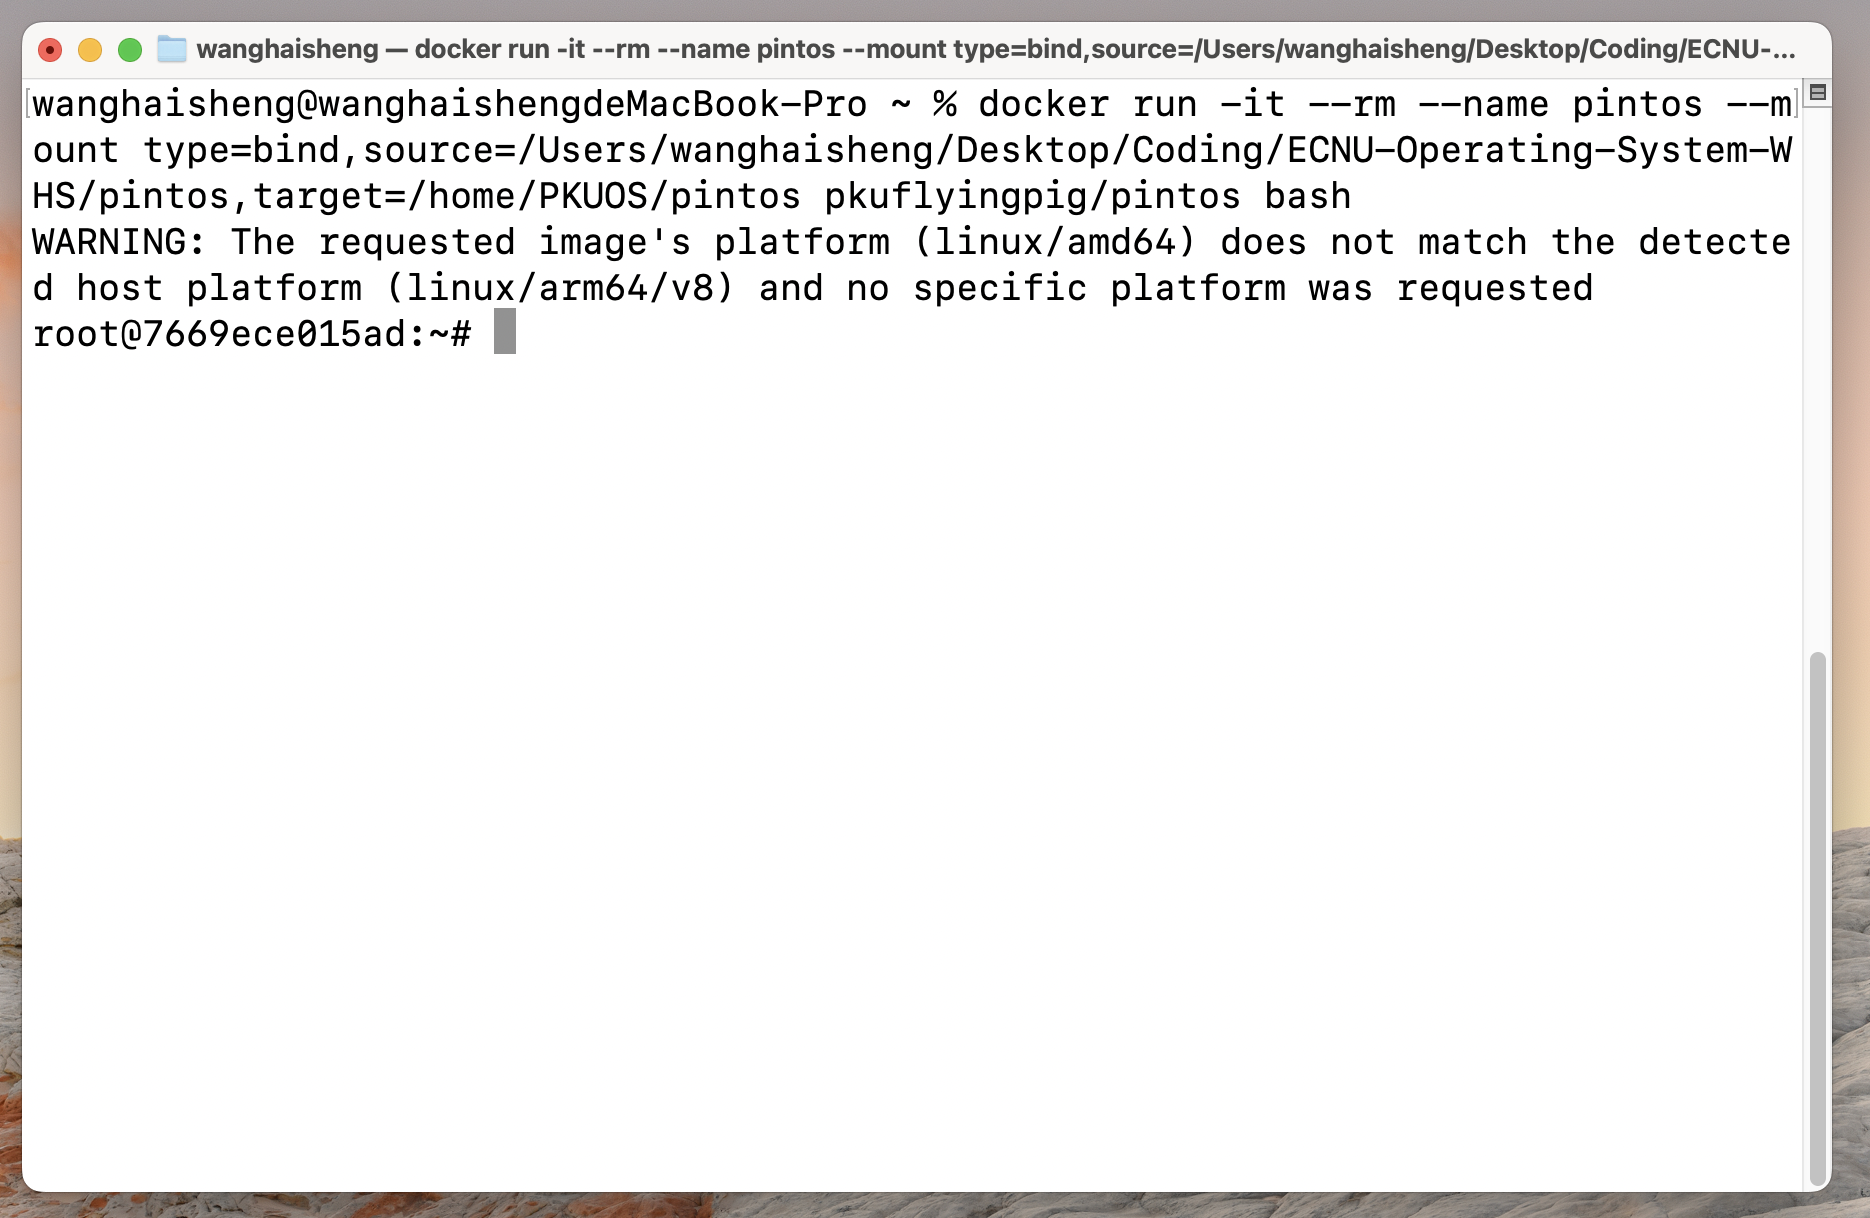
\includegraphics[width=0.9\textwidth]{img/run_docker.png}
	\caption{完成环境配置}
\end{figure}

\normalsize

\section{实验过程}

\subsection{展示忙等}

在\texttt{thread\_yield()}函数中加入打印语句,以便观察线程何时被调度。修改后的\texttt{thread\_yield()}函数如下:

\begin{lstlisting}[language=C, title=\texttt{thread\_yield}]
	void
	thread_yield (void)
	{
		struct thread *cur = thread_current ();
		enum intr_level old_level;
		
		ASSERT (!intr_context ());
		old_level = intr_disable ();
		if (cur != idle_thread)
		list_insert_ordered(&ready_list, &cur->elem, thread_less_priority, NULL);
		printf("Yield: thread(%s) at tick %d.\n", cur->name, timer_ticks());
		// ASSERT(false);
		cur->status = THREAD_READY;
		schedule ();
		intr_set_level (old_level);
	}
\end{lstlisting}

\

运行\texttt{pintos -v -- -q run alarm-multiple}的结果如下所示。可以看到,每个线程在每个时间片结束时都进行了调度,这表明系统正在使用忙等待的方式进行调度,所以效率很低。

\

\begin{lstlisting}
	(alarm-multiple) begin
	(alarm-multiple) Creating 5 threads to sleep 7 times each.
	(alarm-multiple) Thread 0 sleeps 10 ticks each time,
	(alarm-multiple) thread 1 sleeps 20 ticks each time, and so on.
	(alarm-multiple) If successful, product of iteration count and
	(alarm-multiple) sleep duration will appear in nondescending order.
	Yield: thread(main) at tick 26.
	Yield: thread(thread 0) at tick 27.
	Yield: thread(thread 1) at tick 27.
	Yield: thread(thread 2) at tick 27.
	Yield: thread(thread 3) at tick 27.
	Yield: thread(thread 4) at tick 28.
	Yield: thread(main) at tick 28.
	Yield: thread(thread 0) at tick 28.
	Yield: thread(thread 1) at tick 28.
	Yield: thread(thread 2) at tick 28.
	Yield: thread(thread 3) at tick 29.
	Yield: thread(thread 4) at tick 29.
	Yield: thread(main) at tick 29.
	Yield: thread(thread 0) at tick 29.
	Yield: thread(thread 1) at tick 30.
	Yield: thread(thread 2) at tick 30.
	Yield: thread(thread 3) at tick 30.
	Yield: thread(thread 4) at tick 30.
	Yield: thread(main) at tick 31.
	Yield: thread(thread 0) at tick 31.
	Yield: thread(thread 1) at tick 31.
	Yield: thread(thread 2) at tick 31.
	Yield: thread(thread 3) at tick 32.
	Yield: thread(thread 4) at tick 32.
	Yield: thread(main) at tick 32.
	Yield: thread(thread 0) at tick 32.
	Yield: thread(thread 1) at tick 33.
	Yield: thread(thread 2) at tick 33.
	Yield: thread(thread 3) at tick 33.
	Yield: thread(thread 4) at tick 33.
	Yield: thread(main) at tick 34.
\end{lstlisting}

\subsection{实现休眠}

通过对 \texttt{alarm\_wait.c} 测试脚本的分析,我们了解到首先需要创建 \texttt{thread\_cnt} 个进程,每个进程将执行 \texttt{sleeper} 函数。接着,主测试进程会进入休眠状态足够长的时间以确保所有子进程完成它们的任务。在深入研究 \texttt{sleeper} 函数时发现,它调用了 \texttt{timer\_sleep} 函数使每个进程按照 \texttt{iteration} 指定的次数进行休眠,并记录下各个线程被唤醒的顺序。同时,从 \texttt{alarm-zero.c} 和 \texttt{alarm-negative.c} 中了解到还需处理定时器滴答数小于或等于零的情况。

随后,在验证阶段,根据各线程被唤醒的顺序来进行检查,该顺序必须与预期一致;此外,还需确认每个进程确实被唤醒了 \texttt{iteration} 次。只有当这些条件都满足时,才认为整个过程是正确的。

当前面临的主要挑战在于实现 \texttt{timer\_sleep} 函数,特别是需要对其现有的忙等待机制进行改进。

\begin{lstlisting}[language=C, title=\texttt{timer\_sleep}]
	void timer_sleep(int64_t ticks) {
		int64_t start = timer_ticks();
		ASSERT(intr_get_level() == INTR_ON);
		while (timer_elapsed(start) < ticks)
		thread_yield();
	}
\end{lstlisting}

一种实现思路是在每个时钟滴答(tick)检查所有处于等待状态的线程。为此,每个线程需要维护一个名为 \texttt{wait\_ticks} 的变量,用于表示该线程还需要等待多少个时钟滴答。每当发生一次时钟滴答时,遍历整个等待队列,并将每个线程的 \texttt{wait\_ticks} 变量减一。如果某个线程的 \texttt{wait\_ticks} 减至0,则将其从等待队列中移除并添加到就绪队列 \texttt{ready\_list} 中。为了优化性能,可以单独设立一个 \texttt{wait\_list} 专门存放等待中的线程,从而减少每次时钟滴答时需遍历的线程数量。这种方法的插入操作复杂度为 O(1),而处理时钟滴答的操作复杂度为 O(n)。

另一种方法同样使用 \texttt{wait\_list},但每个进程记录的是其预期唤醒的具体时间点。在将新进程加入 \texttt{wait\_list} 时,按照唤醒时间进行排序。这样,在每次时钟滴答时只需要检查 \texttt{wait\_list} 链表头部的进程是否已达到唤醒时间即可。如果条件满足,则将该进程转移到 \texttt{ready\_list}。这种方法的插入操作复杂度为 O(n),而处理时钟滴答的操作复杂度降低到了 O(1)。

考虑到实际应用中,向 \texttt{wait\_list} 插入元素的频率远低于时钟滴答事件发生的频率,因此选择第二种方法更为高效。

\texttt{timer\_sleep} 函数的主要职责是将当前线程放入等待队列,并设置相应的 \texttt{wait\_ticks} 值。可以参考 \texttt{thread\_unblock} 函数来了解如何将线程添加到 \texttt{ready\_list} 的过程,同时借鉴 \texttt{ready\_list} 初始化的方式来初始化 \texttt{wait\_list}。醒来的时间应设定为当前时间加上所需的等待时间。

类似其他涉及进程状态转换的函数,在修改进程状态时必须确保操作的原子性。在 Pintos 操作系统环境中,这通常通过关闭中断来实现。因此,在 \texttt{timer\_sleep} 或类似的 \texttt{thread\_wait} 函数中,应当在关闭中断的状态下完成对进程状态的所有修改。

\begin{lstlisting}[language=C, title=\texttt{thread\_wait}]
	bool thread_less_wake_tick(const struct list_elem *a, const struct list_elem *b, void *aux) {
		int64_t x = list_entry(a, struct thread, waitelem)->wake_tick;
		int64_t y = list_entry(b, struct thread, waitelem)->wake_tick;
		return x < y;
	}
	
	void thread_wait(int64_t wait_ticks) {
		ASSERT(intr_get_level() == INTR_ON);
		enum intr_level old_level = intr_disable();
		int64_t cur_tick = timer_ticks();
		struct thread *t = thread_current();
		t->wake_tick = wait_ticks + cur_tick; // printf("wake_tick:%d\n", t->wake_tick);
		list_insert_ordered(&wait_list, &t->waitelem, thread_less_wake_tick, NULL);
		thread_block();
		intr_set_level(old_level);
	}
	
	void timer_sleep(int64_t ticks) {
		if (ticks <= 0) return;
		thread_wait(ticks);
	}
\end{lstlisting}

接下来的任务是在每个时钟滴答(tick)中唤醒符合条件的线程。可以参考 \texttt{thread\_foreach} 函数来遍历等待队列 \texttt{wait\_list}。当检测到当前系统时间大于或等于某个进程设定的唤醒时间时,该进程应被唤醒,并通过调用 \texttt{thread\_unblock} 函数将其加入到就绪队列 \texttt{ready\_list} 中。同时,从 \texttt{wait\_list} 中移除该进程对应的元素。

由于唤醒时间具有单调递增的特性,一旦遇到一个尚未达到唤醒时间的进程,即可停止继续检查剩余的进程,即在此处使用 \texttt{break} 语句终止循环。这样可以有效地减少不必要的遍历操作,提高效率。

\begin{lstlisting}[language=C, title=\texttt{thread\_unwait}]
	void thread_unwait(void) {
		struct list_elem *e;
		ASSERT(intr_get_level() == INTR_OFF);
		int64_t cur_tick = timer_ticks();
		
		for (e = list_begin(&wait_list); e != list_end(&wait_list); e = list_next(e)) {
			struct thread *t = list_entry(e, struct thread, waitelem);
			if (t->wake_tick > cur_tick) break;
			// printf("wake:%s%d\n", t->name, t->wake_tick);
			list_remove(e);
			thread_unblock(t);
		}
	}
\end{lstlisting}

输出如下, 可以看到每个进程在该醒来的时候就醒来, 不必像忙等待一样时刻都在检查。

\begin{lstlisting}
	Executing 'alarm-multiple':
	(alarm-multiple) begin
	(alarm-multiple) Creating 5 threads to sleep 7 times each.
	(alarm-multiple) Thread 0 sleeps 10 ticks each time,
	(alarm-multiple) thread 1 sleeps 20 ticks each time, and so on.
	(alarm-multiple) If successful, product of iteration count and
	(alarm-multiple) sleep duration will appear in nondescending order.
	wake: thread 0 135
	wake: thread 1 145
	wake: thread 0 145
	wake: thread 2 155
	wake: thread 0 155
	wake: thread 3 165
	wake: thread 1 165
	wake: thread 0 165
	wake: thread 4 175
	wake: thread 0 175
	wake: thread 2 185
	wake: thread 1 185
	wake: thread 0 185
	wake: thread 0 195
	wake: thread 3 205
	wake: thread 1 205
	wake: thread 2 215
	wake: thread 4 225
	wake: thread 1 225
	wake: thread 3 245
	wake: thread 2 245
	wake: thread 1 245
	wake: thread 1 265
	wake: thread 4 275
	wake: thread 2 275
	wake: thread 3 285
	wake: thread 2 305
	wake: thread 4 325
	wake: thread 3 325
	wake: thread 2 335
	wake: thread 3 365
	wake: thread 4 375
	wake: thread 3 405
	wake: thread 4 425
	wake: thread 4 475
	wake: main 575
\end{lstlisting}

\subsection{苏醒后抢占}

当进程从阻塞状态恢复时,可以认为是\texttt{thread\_unwait}通过调用\texttt{thread\_unblock}实现了这一转变。为了确保优先级调整后的正确性,在所有涉及改变优先级的地方适当添加\texttt{thread\_yield}调用。这样处理后,系统就能够顺利通过与优先级相关的测试点。

\begin{lstlisting}[language=C, title=\texttt{thread\_create}]
	tid_t
	thread_create (const char *name, int priority,
	thread_func *function, void *aux)
	{
		//...
		/* Add to run queue. */
		thread_unblock (t);
		thread_yield();
		
		return tid;
	}
	
	void
	thread_set_priority (int new_priority)
	{
		thread_current ()->priority = new_priority;
		thread_yield();
	}
\end{lstlisting}

然而,\texttt{thread\_unwait} 函数是由中断处理程序调用的,在这种情况下当前运行的是 idle 进程,直接调用 \texttt{thread\_yield} 来进行调度是不合适的。通过审查源代码发现,\texttt{intr\_return\_yield} 机制能够满足这一需求。因此,在 \texttt{thread\_unwait} 函数中设置一个标志来指示是否有进程被唤醒,如果确实有进程被唤醒,则在中断返回时利用 \texttt{intr\_return\_yield} 来触发一次调度。

\begin{lstlisting}[language=C, title=\texttt{thread\_unwait}]
	bool thread_unwait()
	{ 
		
		struct list_elem *e;
		ASSERT (intr_get_level () == INTR_OFF);
		int64_t cur_tick = timer_ticks();
		
		bool yield_flag = false;
		
		for (e = list_begin (&wait_list); e != list_end (&wait_list);
		e = list_next (e))
		{
			struct thread *t = list_entry (e, struct thread, waitelem);
			if (t->wake_tick > cur_tick) break;
			
			yield_flag = true;
			list_remove(e);
			thread_unblock(t);
		}
		
		return yield_flag;
	}
\end{lstlisting}

基于之前的实验,我们添加了一个测试脚本,该脚本创建一个高优先级的子进程并使其进入休眠状态,而主进程则进入一个无限循环。当子进程被唤醒后,它应当能够根据其较高的优先级抢占主进程。随后,降低子进程的优先级,这时主进程的循环结束,并且由于优先级调整,尽管此时子进程的优先级更高,但控制权将先返回给主进程。随着子进程的完成,最终主进程也结束运行。以下是具体的测试脚本。

\begin{lstlisting}[language=C, title=测试脚本]
	#include <stdio.h>
	#include "tests/threads/tests.h"
	#include "threads/init.h"
	#include "threads/malloc.h"
	#include "threads/synch.h"
	#include "threads/thread.h"
	#include "devices/timer.h"
	
	static void high_priority_sleeper(void*);
	
	void test_priority_alarm(void) {
		int high_priority = PRI_DEFAULT + 10;
		thread_create("high_priority_sleeper", high_priority, high_priority_sleeper, NULL);
		
		msg("Main thread starts running.");
		int64_t start_tick = timer_ticks();
		while (timer_elapsed(start_tick) < 20);
		
		msg("Main thread thread changed its priority to 21");
		thread_set_priority(21);
		msg("Main thread completed execution.");
	}
	
	static void high_priority_sleeper(void *aux UNUSED) {
		msg("High-priority thread starts and goes to sleep.");
		timer_sleep(10);
		msg("High-priority thread woke up at and preempts the main thread.");
		msg("High-priority thread changed its priority to 26");
		thread_set_priority(PRI_DEFAULT - 5);
		msg("High-priority thread exit.");
	}
	
	void thread_tick(void) {
		struct thread *t = thread_current();
		
		/* Update statistics. */
		if (t == idle_thread)
			idle_ticks++;
		#ifdef USERPROG
		else if (t->pagedir != NULL)
			user_ticks++;
		#endif
		
		else
			kernel_ticks++;
		
		/* Enforce preemption. */
		bool yield_flag = thread_unwait();
		if (++thread_ticks >= TIME_SLICE || yield_flag)
			intr_yield_on_return();
	}
\end{lstlisting}

预期输出如下:

\begin{lstlisting}
	# -*- perl -*-
	use strict;
	use warnings;
	use tests::tests;
	check_expected ([<<'EOF']);
	(priority-alarm) begin
	(priority-alarm) High-priority thread starts and goes to sleep.
	(priority-alarm) Main thread starts running.
	(priority-alarm) High-priority thread woke up at and preempts the main thread.
	(priority-alarm) High-priority thread changed its priority to 26
	(priority-alarm) Main thread thread changed its priority to 21
	(priority-alarm) High-priority thread exit.
	(priority-alarm) Main thread completed execution.
	(priority-alarm) end
	EOF
	pass;
\end{lstlisting}

\normalsize

\section{实验总结}

至此,本实验相关的测试点全部通过,截图如下:

\begin{figure}[H]
	\centering
	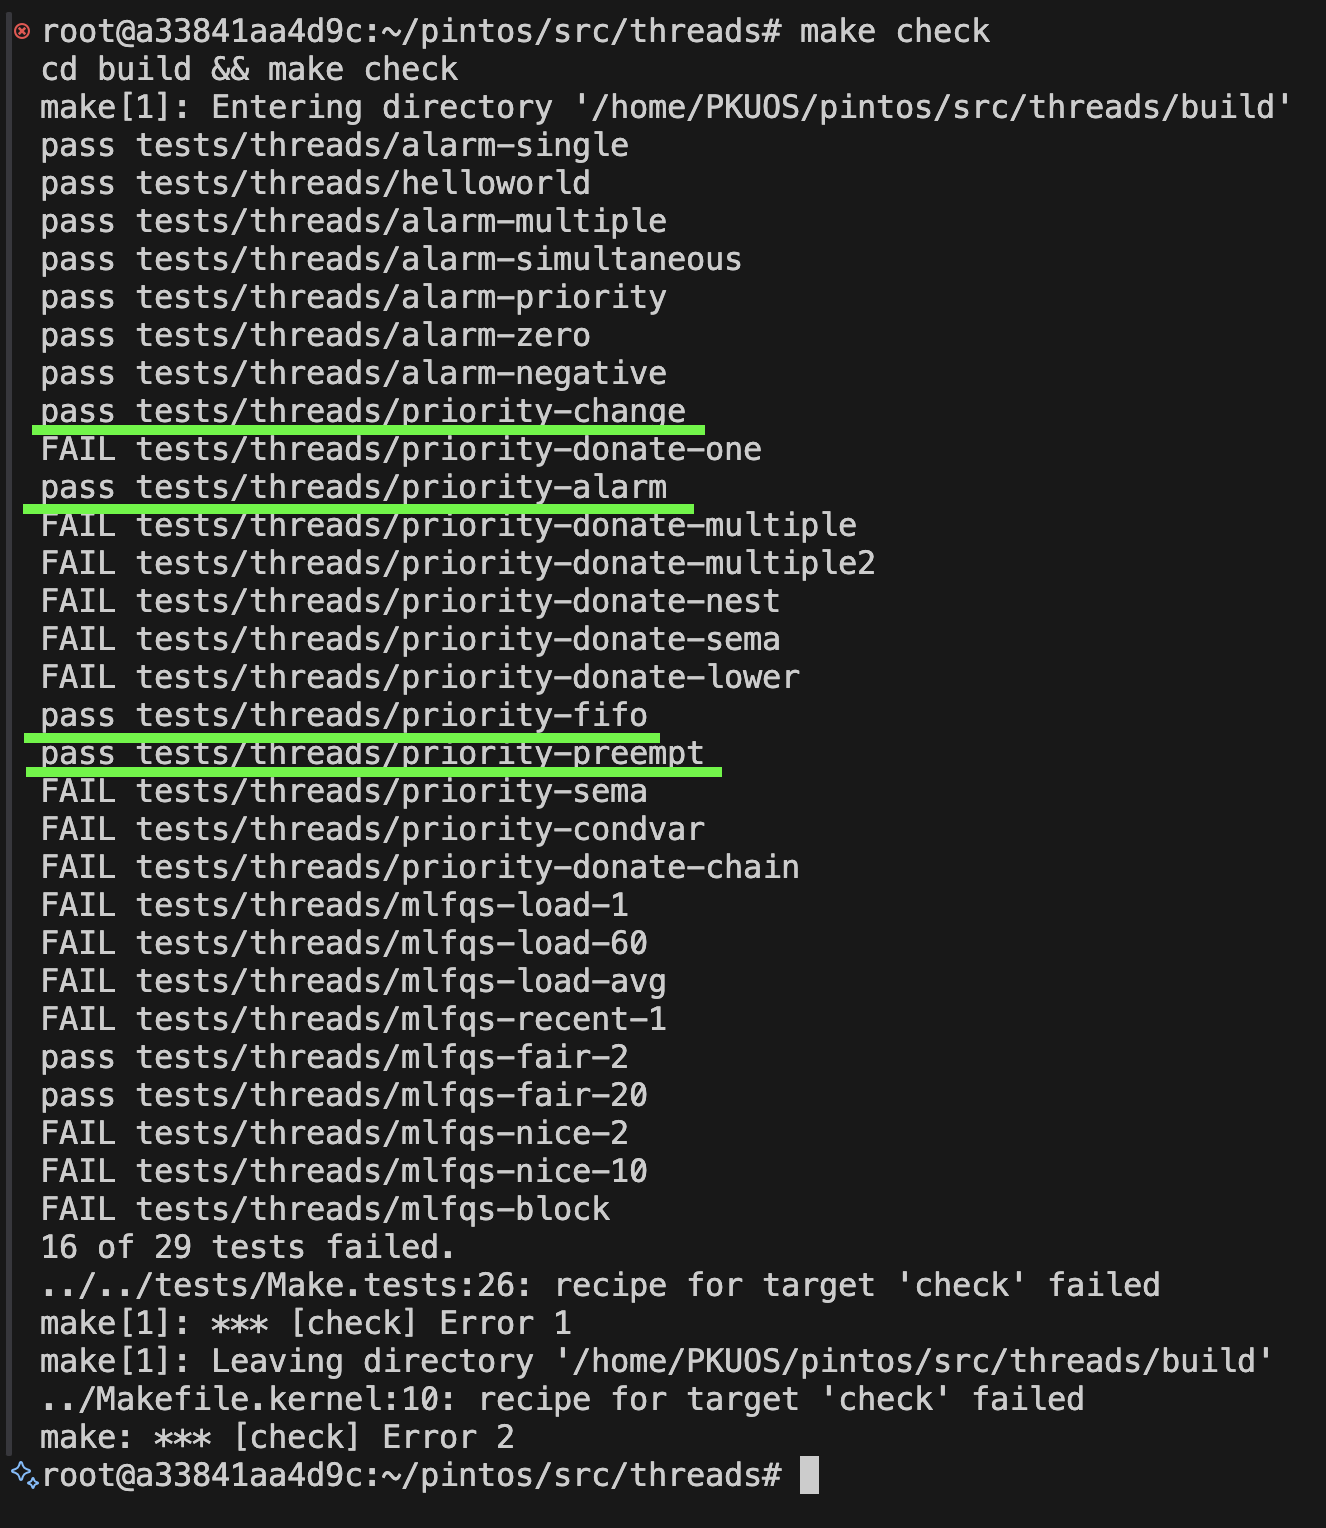
\includegraphics[width=0.9\textwidth]{img/make_check_lab4.png}
	\caption{Docker容器}
\end{figure}

其中,\texttt{priority-alarm}为自定义测试点。

\normalsize

\section{附录:修改后的代码}

\begin{lstlisting}[language=C, title=\texttt{pintos/src/devices/timer.c}]
	#include "devices/timer.h"
	#include <debug.h>
	#include <inttypes.h>
	#include <round.h>
	#include <stdio.h>
	#include "devices/pit.h"
	#include "threads/interrupt.h"
	#include "threads/synch.h"
	#include "threads/thread.h"
	
	/** See [8254] for hardware details of the 8254 timer chip. */
	
	#if TIMER_FREQ < 19
	#error 8254 timer requires TIMER_FREQ >= 19
	#endif
	#if TIMER_FREQ > 1000
	#error TIMER_FREQ <= 1000 recommended
	#endif
	
	/** Number of timer ticks since OS booted. */
	static int64_t ticks;
	
	/** Number of loops per timer tick.
	Initialized by timer_calibrate(). */
	static unsigned loops_per_tick;
	
	static intr_handler_func timer_interrupt;
	static bool too_many_loops (unsigned loops);
	static void busy_wait (int64_t loops);
	static void real_time_sleep (int64_t num, int32_t denom);
	static void real_time_delay (int64_t num, int32_t denom);
	
	/** Sets up the timer to interrupt TIMER_FREQ times per second,
	and registers the corresponding interrupt. */
	void
	timer_init (void) 
	{
		pit_configure_channel (0, 2, TIMER_FREQ);
		intr_register_ext (0x20, timer_interrupt, "8254 Timer");
	}
	
	/** Calibrates loops_per_tick, used to implement brief delays. */
	void
	timer_calibrate (void) 
	{
		unsigned high_bit, test_bit;
		
		ASSERT (intr_get_level () == INTR_ON);
		printf ("Calibrating timer...  ");
		
		/* Approximate loops_per_tick as the largest power-of-two
		still less than one timer tick. */
		loops_per_tick = 1u << 10;
		while (!too_many_loops (loops_per_tick << 1)) 
		{
			loops_per_tick <<= 1;
			ASSERT (loops_per_tick != 0);
		}
		
		/* Refine the next 8 bits of loops_per_tick. */
		high_bit = loops_per_tick;
		for (test_bit = high_bit >> 1; test_bit != high_bit >> 10; test_bit >>= 1)
		if (!too_many_loops (high_bit | test_bit))
		loops_per_tick |= test_bit;
		
		printf ("%'"PRIu64" loops/s.\n", (uint64_t) loops_per_tick * TIMER_FREQ);
	}
	
	/** Returns the number of timer ticks since the OS booted. */
	int64_t
	timer_ticks (void) 
	{
		enum intr_level old_level = intr_disable ();
		int64_t t = ticks;
		intr_set_level (old_level);
		return t;
	}
	
	/** Returns the number of timer ticks elapsed since THEN, which
	should be a value once returned by timer_ticks(). */
	int64_t
	timer_elapsed (int64_t then) 
	{
		return timer_ticks () - then;
	}
	
	/** Sleeps for approximately TICKS timer ticks.  Interrupts must
	be turned on. */
	void
	timer_sleep (int64_t wait_ticks) 
	{
		if (wait_ticks <= 0) return;
		thread_wait(wait_ticks);
		// int64_t start = timer_ticks ();
		
		// ASSERT (intr_get_level () == INTR_ON);
		// while (timer_elapsed (start) < ticks) 
		//   thread_yield ();
		
	}
	
	/** Sleeps for approximately MS milliseconds.  Interrupts must be
	turned on. */
	void
	timer_msleep (int64_t ms) 
	{
		real_time_sleep (ms, 1000);
	}
	
	/** Sleeps for approximately US microseconds.  Interrupts must be
	turned on. */
	void
	timer_usleep (int64_t us) 
	{
		real_time_sleep (us, 1000 * 1000);
	}
	
	/** Sleeps for approximately NS nanoseconds.  Interrupts must be
	turned on. */
	void
	timer_nsleep (int64_t ns) 
	{
		real_time_sleep (ns, 1000 * 1000 * 1000);
	}
	
	/** Busy-waits for approximately MS milliseconds.  Interrupts need
	not be turned on.
	
	Busy waiting wastes CPU cycles, and busy waiting with
	interrupts off for the interval between timer ticks or longer
	will cause timer ticks to be lost.  Thus, use timer_msleep()
	instead if interrupts are enabled. */
	void
	timer_mdelay (int64_t ms) 
	{
		real_time_delay (ms, 1000);
	}
	
	/** Sleeps for approximately US microseconds.  Interrupts need not
	be turned on.
	
	Busy waiting wastes CPU cycles, and busy waiting with
	interrupts off for the interval between timer ticks or longer
	will cause timer ticks to be lost.  Thus, use timer_usleep()
	instead if interrupts are enabled. */
	void
	timer_udelay (int64_t us) 
	{
		real_time_delay (us, 1000 * 1000);
	}
	
	/** Sleeps execution for approximately NS nanoseconds.  Interrupts
	need not be turned on.
	
	Busy waiting wastes CPU cycles, and busy waiting with
	interrupts off for the interval between timer ticks or longer
	will cause timer ticks to be lost.  Thus, use timer_nsleep()
	instead if interrupts are enabled.*/
	void
	timer_ndelay (int64_t ns) 
	{
		real_time_delay (ns, 1000 * 1000 * 1000);
	}
	
	/** Prints timer statistics. */
	void
	timer_print_stats (void) 
	{
		printf ("Timer: %"PRId64" ticks\n", timer_ticks ());
	}
	
	/** Timer interrupt handler. */
	static void
	timer_interrupt (struct intr_frame *args UNUSED)
	{
		ticks++;
		thread_tick ();
	}
	
	/** Returns true if LOOPS iterations waits for more than one timer
	tick, otherwise false. */
	static bool
	too_many_loops (unsigned loops) 
	{
		/* Wait for a timer tick. */
		int64_t start = ticks;
		while (ticks == start)
		barrier ();
		
		/* Run LOOPS loops. */
		start = ticks;
		busy_wait (loops);
		
		/* If the tick count changed, we iterated too long. */
		barrier ();
		return start != ticks;
	}
	
	/** Iterates through a simple loop LOOPS times, for implementing
	brief delays.
	
	Marked NO_INLINE because code alignment can significantly
	affect timings, so that if this function was inlined
	differently in different places the results would be difficult
	to predict. */
	static void NO_INLINE
	busy_wait (int64_t loops) 
	{
		while (loops-- > 0)
		barrier ();
	}
	
	/** Sleep for approximately NUM/DENOM seconds. */
	static void
	real_time_sleep (int64_t num, int32_t denom) 
	{
		/* Convert NUM/DENOM seconds into timer ticks, rounding down.
		
		(NUM / DENOM) s          
		---------------------- = NUM * TIMER_FREQ / DENOM ticks. 
		1 s / TIMER_FREQ ticks
		*/
		int64_t ticks = num * TIMER_FREQ / denom;
		
		ASSERT (intr_get_level () == INTR_ON);
		if (ticks > 0)
		{
			/* We're waiting for at least one full timer tick.  Use
			timer_sleep() because it will yield the CPU to other
			processes. */                
			timer_sleep (ticks); 
		}
		else 
		{
			/* Otherwise, use a busy-wait loop for more accurate
			sub-tick timing. */
			real_time_delay (num, denom); 
		}
	}
	
	/** Busy-wait for approximately NUM/DENOM seconds. */
	static void
	real_time_delay (int64_t num, int32_t denom)
	{
		/* Scale the numerator and denominator down by 1000 to avoid
		the possibility of overflow. */
		ASSERT (denom % 1000 == 0);
		busy_wait (loops_per_tick * num / 1000 * TIMER_FREQ / (denom / 1000)); 
	}	
\end{lstlisting}

\begin{lstlisting}[language=C, title=\texttt{pintos/src/tests/threads/alarm-wait.c}]
	/** Creates N threads, each of which sleeps a different, fixed
	duration, M times.  Records the wake-up order and verifies
	that it is valid. */
	
	#include <stdio.h>
	#include "tests/threads/tests.h"
	#include "threads/init.h"
	#include "threads/malloc.h"
	#include "threads/synch.h"
	#include "threads/thread.h"
	#include "devices/timer.h"
	
	static void test_sleep (int thread_cnt, int iterations);
	
	void
	test_alarm_single (void) 
	{
		test_sleep (5, 1);
	}
	
	void
	test_alarm_multiple (void) 
	{
		test_sleep (5, 7);
	}
	
	/** Information about the test. */
	struct sleep_test 
	{
		int64_t start;              /**< Current time at start of test. */
		int iterations;             /**< Number of iterations per thread. */
		
		/* Output. */
		struct lock output_lock;    /**< Lock protecting output buffer. */
		int *output_pos;            /**< Current position in output buffer. */
	};
	
	/** Information about an individual thread in the test. */
	struct sleep_thread 
	{
		struct sleep_test *test;     /**< Info shared between all threads. */
		int id;                     /**< Sleeper ID. */
		int duration;               /**< Number of ticks to sleep. */
		int iterations;             /**< Iterations counted so far. */
	};
	
	static void sleeper (void *);
	
	/** Runs THREAD_CNT threads thread sleep ITERATIONS times each. */
	static void
	test_sleep (int thread_cnt, int iterations) 
	{
		struct sleep_test test;
		struct sleep_thread *threads;
		int *output, *op;
		int product;
		int i;
		
		/* This test does not work with the MLFQS. */
		ASSERT (!thread_mlfqs);
		msg ("Creating %d threads to sleep %d times each.", thread_cnt, iterations);
		msg ("Thread 0 sleeps 10 ticks each time,");
		msg ("thread 1 sleeps 20 ticks each time, and so on.");
		msg ("If successful, product of iteration count and");
		msg ("sleep duration will appear in nondescending order.");
		/* Allocate memory. */
		threads = malloc (sizeof *threads * thread_cnt);
		output = malloc (sizeof *output * iterations * thread_cnt * 2);
		if (threads == NULL || output == NULL)
		PANIC ("couldn't allocate memory for test");
		
		/* Initialize test. */
		test.start = timer_ticks () + 100;
		test.iterations = iterations;
		lock_init (&test.output_lock);
		test.output_pos = output;
		
		/* Start threads. */
		ASSERT (output != NULL);
		for (i = 0; i < thread_cnt; i++)
		{
			struct sleep_thread *t = threads + i;
			char name[16];
			
			t->test = &test;
			t->id = i;
			t->duration = (i + 1) * 10;
			t->iterations = 0;
			snprintf (name, sizeof name, "thread %d", i);
			thread_create (name, PRI_DEFAULT, sleeper, t);
		}
		
		/* Wait long enough for all the threads to finish. */
		timer_sleep (100 + thread_cnt * iterations * 10 + 100);
		/* Acquire the output lock in case some rogue thread is still
		running. */
		lock_acquire (&test.output_lock);
		
		/* Print completion order. */
		product = 0;
		for (op = output; op < test.output_pos; op++) 
		{
			struct sleep_thread *t;
			int new_prod;
			
			ASSERT (*op >= 0 && *op < thread_cnt);
			t = threads + *op;
			
			new_prod = ++t->iterations * t->duration;
			
			msg ("thread %d: duration=%d, iteration=%d, product=%d",
			t->id, t->duration, t->iterations, new_prod);
			
			if (new_prod >= product)
			product = new_prod;
			else
			fail ("thread %d woke up out of order (%d > %d)!",
			t->id, product, new_prod);
		}
		
		/* Verify that we had the proper number of wakeups. */
		for (i = 0; i < thread_cnt; i++)
		if (threads[i].iterations != iterations)
		fail ("thread %d woke up %d times instead of %d",
		i, threads[i].iterations, iterations);
		
		lock_release (&test.output_lock);
		free (output);
		free (threads);
	}
	
	/** Sleeper thread. */
	static void
	sleeper (void *t_) 
	{
		struct sleep_thread *t = t_;
		struct sleep_test *test = t->test;
		int i;
		
		for (i = 1; i <= test->iterations; i++) 
		{
			int64_t sleep_until = test->start + i * t->duration;
			timer_sleep (sleep_until - timer_ticks ());
			lock_acquire (&test->output_lock);
			*test->output_pos++ = t->id;
			lock_release (&test->output_lock);
		}
	}	
\end{lstlisting}

\begin{lstlisting}[language=C, title=\texttt{pintos/src/tests/threads/priority-alarm.c}]
	#include <stdio.h>
	#include "tests/threads/tests.h"
	#include "threads/init.h"
	#include "threads/malloc.h"
	#include "threads/synch.h"
	#include "threads/thread.h"
	#include "devices/timer.h"
	
	static void high_priority_sleeper(void *);
	
	void test_priority_alarm(void) {
		int high_priority = PRI_DEFAULT + 10;
		thread_create("high_priority_sleeper", high_priority, high_priority_sleeper, NULL);
		
		msg("Main thread starts running.");
		
		int64_t start_tick = timer_ticks();
		while (timer_elapsed(start_tick) < 20);
		
		msg("Main thread thread changed its priority to 21");
		
		thread_set_priority(21);
		
		msg("Main thread completed execution.");
		
	}
	
	static void
	high_priority_sleeper(void *aux UNUSED) {
		msg("High-priority thread starts and goes to sleep.");
		timer_sleep(10);
		msg("High-priority thread woke up at and preempts the main thread.");
		msg("High-priority thread changed its priority to 26");
		thread_set_priority(PRI_DEFAULT - 5);
		msg("High-priority thread exit.");
	}	
\end{lstlisting}

\begin{lstlisting}[title=\texttt{pintos/src/tests/threads/priority-alarm.ck}]
	# -*- perl -*-
	use strict;
	use warnings;
	use tests::tests;
	check_expected ([<<'EOF']);
	(priority-alarm) begin
	(priority-alarm) High-priority thread starts and goes to sleep.
	(priority-alarm) Main thread starts running.
	(priority-alarm) High-priority thread woke up at and preempts the main thread.
	(priority-alarm) High-priority thread changed its priority to 26
	(priority-alarm) Main thread thread changed its priority to 21
	(priority-alarm) High-priority thread exit.
	(priority-alarm) Main thread completed execution.
	(priority-alarm) end
	EOF
	pass;
\end{lstlisting}

\begin{lstlisting}[language=C, title=\texttt{pintos/src/tests/threads/tests.c}]
	#include "tests/threads/tests.h"
	#include <debug.h>
	#include <string.h>
	#include <stdio.h>
	
	struct test 
	{
		const char *name;
		test_func *function;
	};
	
	static const struct test tests[] = 
	{
		{"alarm-single", test_alarm_single},
		{"alarm-multiple", test_alarm_multiple},
		{"alarm-simultaneous", test_alarm_simultaneous},
		{"alarm-priority", test_alarm_priority},
		{"alarm-zero", test_alarm_zero},
		{"alarm-negative", test_alarm_negative},
		{"priority-change", test_priority_change},
		{"priority-donate-one", test_priority_donate_one},
		{"priority-donate-multiple", test_priority_donate_multiple},
		{"priority-donate-multiple2", test_priority_donate_multiple2},
		{"priority-donate-nest", test_priority_donate_nest},
		{"priority-donate-sema", test_priority_donate_sema},
		{"priority-donate-lower", test_priority_donate_lower},
		{"priority-donate-chain", test_priority_donate_chain},
		{"priority-fifo", test_priority_fifo},
		{"priority-preempt", test_priority_preempt},
		{"priority-sema", test_priority_sema},
		{"priority-condvar", test_priority_condvar},
		{"mlfqs-load-1", test_mlfqs_load_1},
		{"mlfqs-load-60", test_mlfqs_load_60},
		{"mlfqs-load-avg", test_mlfqs_load_avg},
		{"mlfqs-recent-1", test_mlfqs_recent_1},
		{"mlfqs-fair-2", test_mlfqs_fair_2},
		{"mlfqs-fair-20", test_mlfqs_fair_20},
		{"mlfqs-nice-2", test_mlfqs_nice_2},
		{"mlfqs-nice-10", test_mlfqs_nice_10},
		{"mlfqs-block", test_mlfqs_block},
		
		
		{"helloworld", test_hello_world},
		{"priority-alarm", test_priority_alarm},
	};
	
	static const char *test_name;
	
	/** Runs the test named NAME. */
	void
	run_test (const char *name) 
	{
		const struct test *t;
		
		for (t = tests; t < tests + sizeof tests / sizeof *tests; t++)
		if (!strcmp (name, t->name))
		{
			test_name = name;
			msg ("begin");
			t->function ();
			msg ("end");
			return;
		}
		PANIC ("no test named \"%s\"", name);
	}
	
	/** Prints FORMAT as if with printf(),
	prefixing the output by the name of the test
	and following it with a new-line character. */
	void
	msg (const char *format, ...) 
	{
		va_list args;
		
		printf ("(%s) ", test_name);
		va_start (args, format);
		vprintf (format, args);
		va_end (args);
		putchar ('\n');
	}
	
	/** Prints failure message FORMAT as if with printf(),
	prefixing the output by the name of the test and FAIL:
	and following it with a new-line character,
	and then panics the kernel. */
	void
	fail (const char *format, ...) 
	{
		va_list args;
		
		printf ("(%s) FAIL: ", test_name);
		va_start (args, format);
		vprintf (format, args);
		va_end (args);
		putchar ('\n');
		
		PANIC ("test failed");
	}
	
	/** Prints a message indicating the current test passed. */
	void
	pass (void) 
	{
		printf ("(%s) PASS\n", test_name);
	}
	
\end{lstlisting}

\begin{lstlisting}[language=C, title=\texttt{pintos/src/tests/threads/tests.h}]
	#ifndef TESTS_THREADS_TESTS_H
	#define TESTS_THREADS_TESTS_H
	
	void run_test (const char *);
	
	typedef void test_func (void);
	
	extern test_func test_alarm_single;
	extern test_func test_alarm_multiple;
	extern test_func test_alarm_simultaneous;
	extern test_func test_alarm_priority;
	extern test_func test_alarm_zero;
	extern test_func test_alarm_negative;
	extern test_func test_priority_change;
	extern test_func test_priority_donate_one;
	extern test_func test_priority_donate_multiple;
	extern test_func test_priority_donate_multiple2;
	extern test_func test_priority_donate_sema;
	extern test_func test_priority_donate_nest;
	extern test_func test_priority_donate_lower;
	extern test_func test_priority_donate_chain;
	extern test_func test_priority_fifo;
	extern test_func test_priority_preempt;
	extern test_func test_priority_sema;
	extern test_func test_priority_condvar;
	extern test_func test_mlfqs_load_1;
	extern test_func test_mlfqs_load_60;
	extern test_func test_mlfqs_load_avg;
	extern test_func test_mlfqs_recent_1;
	extern test_func test_mlfqs_fair_2;
	extern test_func test_mlfqs_fair_20;
	extern test_func test_mlfqs_nice_2;
	extern test_func test_mlfqs_nice_10;
	extern test_func test_mlfqs_block;
	extern test_func test_priority_alarm;
	
	extern test_func test_hello_world;
	
	void msg (const char *, ...);
	void fail (const char *, ...);
	void pass (void);
	
	#endif /**< tests/threads/tests.h */
	
\end{lstlisting}

\begin{lstlisting}[language=C, title=\texttt{pintos/src/threads/thread.c}]
	#include "threads/thread.h"
	#include <debug.h>
	#include <stddef.h>
	#include <random.h>
	#include <stdio.h>
	#include <string.h>
	#include "threads/flags.h"
	#include "threads/interrupt.h"
	#include "threads/intr-stubs.h"
	#include "threads/palloc.h"
	#include "threads/switch.h"
	#include "threads/synch.h"
	#include "threads/vaddr.h"
	#ifdef USERPROG
	#include "userprog/process.h"
	#endif
	
	/** Random value for struct thread's `magic' member.
	Used to detect stack overflow.  See the big comment at the top
	of thread.h for details. */
	#define THREAD_MAGIC 0xcd6abf4b
	
	static struct list wait_list;
	/** List of processes in THREAD_READY state, that is, processes
	that are ready to run but not actually running. */
	static struct list ready_list;
	
	/** List of all processes.  Processes are added to this list
	when they are first scheduled and removed when they exit. */
	static struct list all_list;
	
	/** Idle thread. */
	static struct thread *idle_thread;
	
	/** Initial thread, the thread running init.c:main(). */
	static struct thread *initial_thread;
	
	/** Lock used by allocate_tid(). */
	static struct lock tid_lock;
	
	/** Stack frame for kernel_thread(). */
	struct kernel_thread_frame 
	{
		void *eip;                  /**< Return address. */
		thread_func *function;      /**< Function to call. */
		void *aux;                  /**< Auxiliary data for function. */
	};
	
	/** Statistics. */
	static long long idle_ticks;    /**< # of timer ticks spent idle. */
	static long long kernel_ticks;  /**< # of timer ticks in kernel threads. */
	static long long user_ticks;    /**< # of timer ticks in user programs. */
	
	/** Scheduling. */
	#define TIME_SLICE 4            /**< # of timer ticks to give each thread. */
	static unsigned thread_ticks;   /**< # of timer ticks since last yield. */
	
	/** If false (default), use round-robin scheduler.
	If true, use multi-level feedback queue scheduler.
	Controlled by kernel command-line option "-o mlfqs". */
	bool thread_mlfqs;
	
	static void kernel_thread (thread_func *, void *aux);
	
	static void idle (void *aux UNUSED);
	static struct thread *running_thread (void);
	static struct thread *next_thread_to_run (void);
	static void init_thread (struct thread *, const char *name, int priority);
	static bool is_thread (struct thread *) UNUSED;
	static void *alloc_frame (struct thread *, size_t size);
	static void schedule (void);
	void thread_schedule_tail (struct thread *prev);
	static tid_t allocate_tid (void);
	bool thread_more_priority (const struct list_elem *a,
	const struct list_elem *b,
	void *aux);
	
	bool thread_less_wake_tick(const struct list_elem *a,
	const struct list_elem *b,
	void *aux);
	
	/** Initializes the threading system by transforming the code
	that's currently running into a thread.  This can't work in
	general and it is possible in this case only because loader.S
	was careful to put the bottom of the stack at a page boundary.
	
	Also initializes the run queue and the tid lock.
	
	After calling this function, be sure to initialize the page
	allocator before trying to create any threads with
	thread_create().
	
	It is not safe to call thread_current() until this function
	finishes. */
	void
	thread_init (void) 
	{
		ASSERT (intr_get_level () == INTR_OFF);
		
		lock_init (&tid_lock);
		list_init (&ready_list);
		list_init (&wait_list);
		list_init (&all_list);
		
		/* Set up a thread structure for the running thread. */
		initial_thread = running_thread ();
		init_thread (initial_thread, "main", PRI_DEFAULT);
		initial_thread->status = THREAD_RUNNING;
		initial_thread->tid = allocate_tid ();
	}
	
	/** Starts preemptive thread scheduling by enabling interrupts.
	Also creates the idle thread. */
	void
	thread_start (void) 
	{
		/* Create the idle thread. */
		struct semaphore idle_started;
		sema_init (&idle_started, 0);
		thread_create ("idle", PRI_MIN, idle, &idle_started);
		/* Start preemptive thread scheduling. */
		intr_enable ();
		
		/* Wait for the idle thread to initialize idle_thread. */
		sema_down (&idle_started);
	}
	
	/** Called by the timer interrupt handler at each timer tick.
	Thus, this function runs in an external interrupt context. */
	void
	thread_tick (void) 
	{
		struct thread *t = thread_current ();
		
		/* Update statistics. */
		if (t == idle_thread)
		idle_ticks++;
		#ifdef USERPROG
		else if (t->pagedir != NULL)
		user_ticks++;
		#endif
		else
		kernel_ticks++;
		
		/* Enforce preemption. */
		bool yield_flag = thread_unwait();
		if (++thread_ticks >= TIME_SLICE || yield_flag)
		intr_yield_on_return ();
	}
	
	/** Prints thread statistics. */
	void
	thread_print_stats (void) 
	{
		printf ("Thread: %lld idle ticks, %lld kernel ticks, %lld user ticks\n",
		idle_ticks, kernel_ticks, user_ticks);
	}
	
	/** Creates a new kernel thread named NAME with the given initial
	PRIORITY, which executes FUNCTION passing AUX as the argument,
	and adds it to the ready queue.  Returns the thread identifier
	for the new thread, or TID_ERROR if creation fails.
	
	If thread_start() has been called, then the new thread may be
	scheduled before thread_create() returns.  It could even exit
	before thread_create() returns.  Contrariwise, the original
	thread may run for any amount of time before the new thread is
	scheduled.  Use a semaphore or some other form of
	synchronization if you need to ensure ordering.
	
	The code provided sets the new thread's `priority' member to
	PRIORITY, but no actual priority scheduling is implemented.
	Priority scheduling is the goal of Problem 1-3. */
	tid_t
	thread_create (const char *name, int priority,
	thread_func *function, void *aux) 
	{
		struct thread *t;
		struct kernel_thread_frame *kf;
		struct switch_entry_frame *ef;
		struct switch_threads_frame *sf;
		tid_t tid;
		
		ASSERT (function != NULL);
		
		/* Allocate thread. */
		t = palloc_get_page (PAL_ZERO);
		if (t == NULL)
		return TID_ERROR;
		
		/* Initialize thread. */
		init_thread (t, name, priority);
		tid = t->tid = allocate_tid ();
		
		/* Stack frame for kernel_thread(). */
		kf = alloc_frame (t, sizeof *kf);
		kf->eip = NULL;
		kf->function = function;
		kf->aux = aux;
		
		/* Stack frame for switch_entry(). */
		ef = alloc_frame (t, sizeof *ef);
		ef->eip = (void (*) (void)) kernel_thread;
		
		/* Stack frame for switch_threads(). */
		sf = alloc_frame (t, sizeof *sf);
		sf->eip = switch_entry;
		sf->ebp = 0;
		
		/* Add to run queue. */
		thread_unblock (t);
		thread_yield();
		
		return tid;
	}
	
	/** Puts the current thread to sleep.  It will not be scheduled
	again until awoken by thread_unblock().
	
	This function must be called with interrupts turned off.  It
	is usually a better idea to use one of the synchronization
	primitives in synch.h. */
	void
	thread_block (void) 
	{
		ASSERT (!intr_context ());
		ASSERT (intr_get_level () == INTR_OFF);
		
		thread_current ()->status = THREAD_BLOCKED;
		schedule ();
	}
	
	bool thread_unwait()
	{  
		
		struct list_elem *e;
		ASSERT (intr_get_level () == INTR_OFF);
		int64_t cur_tick = timer_ticks();
		
		bool yield_flag = false;
		
		for (e = list_begin (&wait_list); e != list_end (&wait_list);
		e = list_next (e))
		{
			struct thread *t = list_entry (e, struct thread, waitelem);
			if (t->wake_tick > cur_tick) break;
			
			yield_flag = true;
			list_remove(e);
			thread_unblock(t);
		}
		
		return yield_flag;
	}
	
	
	/** Transitions a blocked thread T to the ready-to-run state.
	This is an error if T is not blocked.  (Use thread_yield() to
	make the running thread ready.)
	
	This function does not preempt the running thread.  This can
	be important: if the caller had disabled interrupts itself,
	it may expect that it can atomically unblock a thread and
	update other data. */
	void
	thread_unblock (struct thread *t) 
	{
		enum intr_level old_level;
		
		ASSERT (is_thread (t));
		
		old_level = intr_disable ();
		ASSERT (t->status == THREAD_BLOCKED);
		list_insert_ordered(&ready_list, &t->elem, thread_more_priority, NULL);
		// list_push_back (&ready_list, &t->elem);
		t->status = THREAD_READY;
		intr_set_level (old_level);
	}
	
	
	void thread_wait(int64_t wait_ticks) 
	{
		
		ASSERT(intr_get_level() == INTR_ON);
		enum intr_level old_level = intr_disable();
		int64_t cur_tick = timer_ticks();
		struct thread* t = thread_current();
		t->wake_tick = wait_ticks + cur_tick;
		// printf("wake_tick: %d\n", t->wake_tick);
		
		list_insert_ordered(&wait_list, &t->waitelem, thread_less_wake_tick, NULL);
		thread_block();
		
		intr_set_level(old_level);
	}
	
	/** Returns the name of the running thread. */
	const char *
	thread_name (void) 
	{
		return thread_current ()->name;
	}
	
	/** Returns the running thread.
	This is running_thread() plus a couple of sanity checks.
	See the big comment at the top of thread.h for details. */
	struct thread *
	thread_current (void) 
	{
		struct thread *t = running_thread ();
		
		/* Make sure T is really a thread.
		If either of these assertions fire, then your thread may
		have overflowed its stack.  Each thread has less than 4 kB
		of stack, so a few big automatic arrays or moderate
		recursion can cause stack overflow. */
		ASSERT (is_thread (t));
		ASSERT (t->status == THREAD_RUNNING);
		
		return t;
	}
	
	/** Returns the running thread's tid. */
	tid_t
	thread_tid (void) 
	{
		return thread_current ()->tid;
	}
	
	/** Deschedules the current thread and destroys it.  Never
	returns to the caller. */
	void
	thread_exit (void) 
	{
		ASSERT (!intr_context ());
		
		#ifdef USERPROG
		process_exit ();
		#endif
		
		/* Remove thread from all threads list, set our status to dying,
		and schedule another process.  That process will destroy us
		when it calls thread_schedule_tail(). */
		intr_disable ();
		list_remove (&thread_current()->allelem);
		thread_current ()->status = THREAD_DYING;
		schedule ();
		NOT_REACHED ();
	}
	
	/** Yields the CPU.  The current thread is not put to sleep and
	may be scheduled again immediately at the scheduler's whim. */
	void
	thread_yield (void) 
	{
		struct thread *cur = thread_current ();
		enum intr_level old_level;
		
		ASSERT (!intr_context ());
		
		old_level = intr_disable ();
		if (cur != idle_thread) 
		list_insert_ordered(&ready_list, &cur->elem, thread_more_priority, NULL);
		// list_push_back (&ready_list, &cur->elem);
		// ASSERT(false);
		cur->status = THREAD_READY;
		schedule ();
		intr_set_level (old_level);
	}
	
	/** Invoke function 'func' on all threads, passing along 'aux'.
	This function must be called with interrupts off. */
	void
	thread_foreach (thread_action_func *func, void *aux)
	{
		struct list_elem *e;
		
		ASSERT (intr_get_level () == INTR_OFF);
		
		for (e = list_begin (&all_list); e != list_end (&all_list);
		e = list_next (e))
		{
			struct thread *t = list_entry (e, struct thread, allelem);
			func (t, aux);
		}
	}
	
	/** Sets the current thread's priority to NEW_PRIORITY. */
	void
	thread_set_priority (int new_priority) 
	{
		thread_current ()->priority = new_priority;
		thread_yield();
	}
	
	/** Returns the current thread's priority. */
	int
	thread_get_priority (void) 
	{
		return thread_current ()->priority;
	}
	
	/** Sets the current thread's nice value to NICE. */
	void
	thread_set_nice (int nice UNUSED) 
	{
		/* Not yet implemented. */
	}
	
	/** Returns the current thread's nice value. */
	int
	thread_get_nice (void) 
	{
		/* Not yet implemented. */
		return 0;
	}
	
	/** Returns 100 times the system load average. */
	int
	thread_get_load_avg (void) 
	{
		/* Not yet implemented. */
		return 0;
	}
	
	/** Returns 100 times the current thread's recent_cpu value. */
	int
	thread_get_recent_cpu (void) 
	{
		/* Not yet implemented. */
		return 0;
	}
	
	/** Idle thread.  Executes when no other thread is ready to run.
	
	The idle thread is initially put on the ready list by
	thread_start().  It will be scheduled once initially, at which
	point it initializes idle_thread, "up"s the semaphore passed
	to it to enable thread_start() to continue, and immediately
	blocks.  After that, the idle thread never appears in the
	ready list.  It is returned by next_thread_to_run() as a
	special case when the ready list is empty. */
	static void
	idle (void *idle_started_ UNUSED) 
	{
		struct semaphore *idle_started = idle_started_;
		idle_thread = thread_current ();
		sema_up (idle_started);
		
		for (;;) 
		{
			/* Let someone else run. */
			intr_disable ();
			thread_block ();
			
			/* Re-enable interrupts and wait for the next one.
			
			The `sti' instruction disables interrupts until the
			completion of the next instruction, so these two
			instructions are executed atomically.  This atomicity is
			important; otherwise, an interrupt could be handled
			between re-enabling interrupts and waiting for the next
			one to occur, wasting as much as one clock tick worth of
			time.
			
			See [IA32-v2a] "HLT", [IA32-v2b] "STI", and [IA32-v3a]
			7.11.1 "HLT Instruction". */
			asm volatile ("sti; hlt" : : : "memory");
		}
	}
	
	/** Function used as the basis for a kernel thread. */
	static void
	kernel_thread (thread_func *function, void *aux) 
	{
		ASSERT (function != NULL);
		
		intr_enable ();       /**< The scheduler runs with interrupts off. */
		function (aux);       /**< Execute the thread function. */
		thread_exit ();       /**< If function() returns, kill the thread. */
	}
	
	/** Returns the running thread. */
	struct thread *
	running_thread (void) 
	{
		uint32_t *esp;
		
		/* Copy the CPU's stack pointer into `esp', and then round that
		down to the start of a page.  Because `struct thread' is
		always at the beginning of a page and the stack pointer is
		somewhere in the middle, this locates the curent thread. */
		asm ("mov %%esp, %0" : "=g" (esp));
		return pg_round_down (esp);
	}
	
	/** Returns true if T appears to point to a valid thread. */
	static bool
	is_thread (struct thread *t)
	{
		return t != NULL && t->magic == THREAD_MAGIC;
	}
	
	/** Does basic initialization of T as a blocked thread named
	NAME. */
	static void
	init_thread (struct thread *t, const char *name, int priority)
	{
		enum intr_level old_level;
		
		ASSERT (t != NULL);
		ASSERT (PRI_MIN <= priority && priority <= PRI_MAX);
		ASSERT (name != NULL);
		
		memset (t, 0, sizeof *t);
		t->status = THREAD_BLOCKED;
		strlcpy (t->name, name, sizeof t->name);
		t->stack = (uint8_t *) t + PGSIZE;
		t->priority = priority;
		t->magic = THREAD_MAGIC;
		t->wake_tick = -1;
		
		old_level = intr_disable ();
		
		list_insert_ordered(&all_list, &t->allelem, thread_more_priority, NULL);
		// list_push_back (&all_list, &t->allelem);
		intr_set_level (old_level);
	}
	
	/** Allocates a SIZE-byte frame at the top of thread T's stack and
	returns a pointer to the frame's base. */
	static void *
	alloc_frame (struct thread *t, size_t size) 
	{
		/* Stack data is always allocated in word-size units. */
		ASSERT (is_thread (t));
		ASSERT (size % sizeof (uint32_t) == 0);
		
		t->stack -= size;
		return t->stack;
	}
	
	/** Chooses and returns the next thread to be scheduled.  Should
	return a thread from the run queue, unless the run queue is
	empty.  (If the running thread can continue running, then it
	will be in the run queue.)  If the run queue is empty, return
	idle_thread. */
	static struct thread *
	next_thread_to_run (void) 
	{
		if (list_empty (&ready_list))
		return idle_thread;
		else
		return list_entry (list_pop_front (&ready_list), struct thread, elem);
	}
	
	/** Completes a thread switch by activating the new thread's page
	tables, and, if the previous thread is dying, destroying it.
	
	At this function's invocation, we just switched from thread
	PREV, the new thread is already running, and interrupts are
	still disabled.  This function is normally invoked by
	thread_schedule() as its final action before returning, but
	the first time a thread is scheduled it is called by
	switch_entry() (see switch.S).
	
	It's not safe to call printf() until the thread switch is
	complete.  In practice that means that printf()s should be
	added at the end of the function.
	
	After this function and its caller returns, the thread switch
	is complete. */
	void
	thread_schedule_tail (struct thread *prev)
	{
		struct thread *cur = running_thread ();
		
		ASSERT (intr_get_level () == INTR_OFF);
		
		/* Mark us as running. */
		cur->status = THREAD_RUNNING;
		
		/* Start new time slice. */
		thread_ticks = 0;
		
		#ifdef USERPROG
		/* Activate the new address space. */
		process_activate ();
		#endif
		
		/* If the thread we switched from is dying, destroy its struct
		thread.  This must happen late so that thread_exit() doesn't
		pull out the rug under itself.  (We don't free
		initial_thread because its memory was not obtained via
		palloc().) */
		if (prev != NULL && prev->status == THREAD_DYING && prev != initial_thread) 
		{
			ASSERT (prev != cur);
			palloc_free_page (prev);
		}
	}
	
	/** Schedules a new process.  At entry, interrupts must be off and
	the running process's state must have been changed from
	running to some other state.  This function finds another
	thread to run and switches to it.
	
	It's not safe to call printf() until thread_schedule_tail()
	has completed. */
	static void
	schedule (void) 
	{
		struct thread *cur = running_thread ();
		struct thread *next = next_thread_to_run ();
		struct thread *prev = NULL;
		
		ASSERT (intr_get_level () == INTR_OFF);
		ASSERT (cur->status != THREAD_RUNNING);
		ASSERT (is_thread (next));
		
		if (cur != next)
		prev = switch_threads (cur, next);
		thread_schedule_tail (prev);
	}
	
	/** Returns a tid to use for a new thread. */
	static tid_t
	allocate_tid (void) 
	{
		static tid_t next_tid = 1;
		tid_t tid;
		
		lock_acquire (&tid_lock);
		tid = next_tid++;
		lock_release (&tid_lock);
		
		return tid;
	}
	
	/** Offset of `stack' member within `struct thread'.
	Used by switch.S, which can't figure it out on its own. */
	uint32_t thread_stack_ofs = offsetof (struct thread, stack);
	
	bool thread_more_priority (const struct list_elem *a,
	const struct list_elem *b,
	void *aux) 
	{
		int x = list_entry(a, struct thread, elem)->priority;
		int y = list_entry(b, struct thread, elem)->priority;
		return x > y;
	}
	
	bool thread_less_wake_tick(const struct list_elem *a,
	const struct list_elem *b,
	void *aux) 
	{
		int64_t x = list_entry(a, struct thread, waitelem)->wake_tick;
		int64_t y = list_entry(b, struct thread, waitelem)->wake_tick;
		return x < y;
	}
\end{lstlisting}

\begin{lstlisting}[language=C, title=\texttt{pintos/src/threads/thread.h}]
	#ifndef THREADS_THREAD_H
	#define THREADS_THREAD_H
	
	#include <debug.h>
	#include <list.h>
	#include <stdint.h>
	
	/** States in a thread's life cycle. */
	enum thread_status
	{
		THREAD_RUNNING,     /**< Running thread. */
		THREAD_READY,       /**< Not running but ready to run. */
		THREAD_BLOCKED,     /**< Waiting for an event to trigger. */
		THREAD_DYING        /**< About to be destroyed. */
	};
	
	/** Thread identifier type.
	You can redefine this to whatever type you like. */
	typedef int tid_t;
	#define TID_ERROR ((tid_t) -1)          /**< Error value for tid_t. */
	
	/** Thread priorities. */
	#define PRI_MIN 0                       /**< Lowest priority. */
	#define PRI_DEFAULT 31                  /**< Default priority. */
	#define PRI_MAX 63                      /**< Highest priority. */
	
	/** A kernel thread or user process.
	
	Each thread structure is stored in its own 4 kB page.  The
	thread structure itself sits at the very bottom of the page
	(at offset 0).  The rest of the page is reserved for the
	thread's kernel stack, which grows downward from the top of
	the page (at offset 4 kB).  Here's an illustration:
	
	4 kB +---------------------------------+
	|          kernel stack           |
	|                |                |
	|                |                |
	|                V                |
	|         grows downward          |
	|                                 |
	|                                 |
	|                                 |
	|                                 |
	|                                 |
	|                                 |
	|                                 |
	|                                 |
	+---------------------------------+
	|              magic              |
	|                :                |
	|                :                |
	|               name              |
	|              status             |
	0 kB +---------------------------------+
	
	The upshot of this is twofold:
	
	1. First, `struct thread' must not be allowed to grow too
	big.  If it does, then there will not be enough room for
	the kernel stack.  Our base `struct thread' is only a
	few bytes in size.  It probably should stay well under 1
	kB.
	
	2. Second, kernel stacks must not be allowed to grow too
	large.  If a stack overflows, it will corrupt the thread
	state.  Thus, kernel functions should not allocate large
	structures or arrays as non-static local variables.  Use
	dynamic allocation with malloc() or palloc_get_page()
	instead.
	
	The first symptom of either of these problems will probably be
	an assertion failure in thread_current(), which checks that
	the `magic' member of the running thread's `struct thread' is
	set to THREAD_MAGIC.  Stack overflow will normally change this
	value, triggering the assertion. */
	/** The `elem' member has a dual purpose.  It can be an element in
	the run queue (thread.c), or it can be an element in a
	semaphore wait list (synch.c).  It can be used these two ways
	only because they are mutually exclusive: only a thread in the
	ready state is on the run queue, whereas only a thread in the
	blocked state is on a semaphore wait list. */
	struct thread
	{
		/* Owned by thread.c. */
		tid_t tid;                          /**< Thread identifier. */
		enum thread_status status;          /**< Thread state. */
		char name[16];                      /**< Name (for debugging purposes). */
		uint8_t *stack;                     /**< Saved stack pointer. */
		int priority;                       /**< Priority. */
		struct list_elem allelem;           /**< List element for all threads list. */
		
		struct list_elem waitelem;
		int64_t wake_tick;
		
		/* Shared between thread.c and synch.c. */
		struct list_elem elem;              /**< List element. */
		
		#ifdef USERPROG
		/* Owned by userprog/process.c. */
		uint32_t *pagedir;                  /**< Page directory. */
		#endif
		
		/* Owned by thread.c. */
		unsigned magic;                     /**< Detects stack overflow. */
	};
	
	/** If false (default), use round-robin scheduler.
	If true, use multi-level feedback queue scheduler.
	Controlled by kernel command-line option "-o mlfqs". */
	extern bool thread_mlfqs;
	
	void thread_init (void);
	void thread_start (void);
	
	void thread_tick (void);
	void thread_print_stats (void);
	
	typedef void thread_func (void *aux);
	tid_t thread_create (const char *name, int priority, thread_func *, void *);
	
	void thread_block (void);
	void thread_unblock (struct thread *);
	void thread_wait(int64_t ticks);
	bool thread_unwait();
	
	struct thread *thread_current (void);
	tid_t thread_tid (void);
	const char *thread_name (void);
	
	void thread_exit (void) NO_RETURN;
	void thread_yield (void);
	
	/** Performs some operation on thread t, given auxiliary data AUX. */
	typedef void thread_action_func (struct thread *t, void *aux);
	void thread_foreach (thread_action_func *, void *);
	
	int thread_get_priority (void);
	void thread_set_priority (int);
	
	int thread_get_nice (void);
	void thread_set_nice (int);
	int thread_get_recent_cpu (void);
	int thread_get_load_avg (void);
	
	#endif /**< threads/thread.h */
\end{lstlisting}

\normalsize

\end{document}